\appendix

% --- PDF will be split by an editor (e.g. macOS preview), so need to restart from page 1
\setcounter{page}{1}

% --- repeat the title (AT: haven't found a more elegant way to do this...)
\twocolumn[
\centering
\Large
% \textbf{[CVPR2022] Official LaTeX Template} \\
\textbf{Supplementary Material} \\
\vspace{1.0em}
] %< twocolumn

\appendix

\definecolor{lightblue}{rgb}{0.63, 0.74, 0.78}
\definecolor{seagreen}{rgb}{0.18, 0.42, 0.41}
\definecolor{orange}{rgb}{0.85, 0.55, 0.13}
\definecolor{silver}{rgb}{0.69, 0.67, 0.66}
\definecolor{rust}{rgb}{0.72, 0.26, 0.06}

\colorlet{lightsilver}{silver!30!white}
\colorlet{darkorange}{orange!75!black}
\colorlet{darksilver}{silver!65!black}
\colorlet{darklightblue}{lightblue!65!black}
\colorlet{darkrust}{rust!85!black}

\tikzstyle{trainingstyle} = [rectangle, 
minimum width=2cm, 
minimum height=2cm,
text centered,
text width=1.5cm,
draw=black,
thick,
rounded corners=0.3cm, 
fill=lightsilver, label=(a)]


\tikzstyle{onnxstyle} = [rectangle, 
minimum width=2cm, 
minimum height=0.8cm, 
text centered,
draw=black, 
thick,
rotate=90,
rounded corners=0.3cm,
fill=lightsilver, label=right:(b)]

\tikzstyle{mtestyle} = [rectangle, 
minimum width=2.7cm, 
minimum height=0.8cm, 
text centered, 
text width=2.8cm,
thick,
draw=black, 
rotate=90,
thick,
rounded corners=0.3cm,
fill=lightsilver, label=right:(d)]

\tikzstyle{decodingstyle} = [rectangle, 
minimum width=2cm, 
minimum height=0.8cm, 
text centered,
draw=black,
rotate=0,
thick,
rounded corners=0.3cm,
fill=rust!30, label=(f)]

\tikzstyle{eucstyle} = [rectangle, 
minimum width=2cm, 
minimum height=1cm,
text centered,
text width=1.55cm,
draw=black,
thick,
rounded corners=0.3cm, 
fill=white, label={[xshift=0.15cm]right:(g)}]

\tikzstyle{border1style} = [rectangle, 
minimum width=2.5cm, 
minimum height=4.75cm,
text centered,
text depth=4cm,
draw=black,
rounded corners=0.3cm, 
thick,
fill=lightsilver,
fill opacity=1, label={[xshift=0.5cm]above:(e)}]

\tikzstyle{border2style} = [rectangle, 
minimum width=4.5cm, 
minimum height=4cm,
text centered,
text depth=3.5cm,
draw=black,
dashed,
very thick,
rounded corners=0.3cm, 
fill=seagreen,
fill opacity=0.1,
text opacity=1,
label=(c)]

\tikzstyle{hpcstyle} = [rectangle, 
minimum width=2cm, 
minimum height=2cm,
text centered,
text width=1.9cm,
draw=black,
thick,
rounded corners=0.3cm, 
fill=lightsilver, label=(h)]

\tikzstyle{arrow} = [very thick,->,>=latex]
\tikzstyle{darrow} = [very thick,<->,>=latex]
    
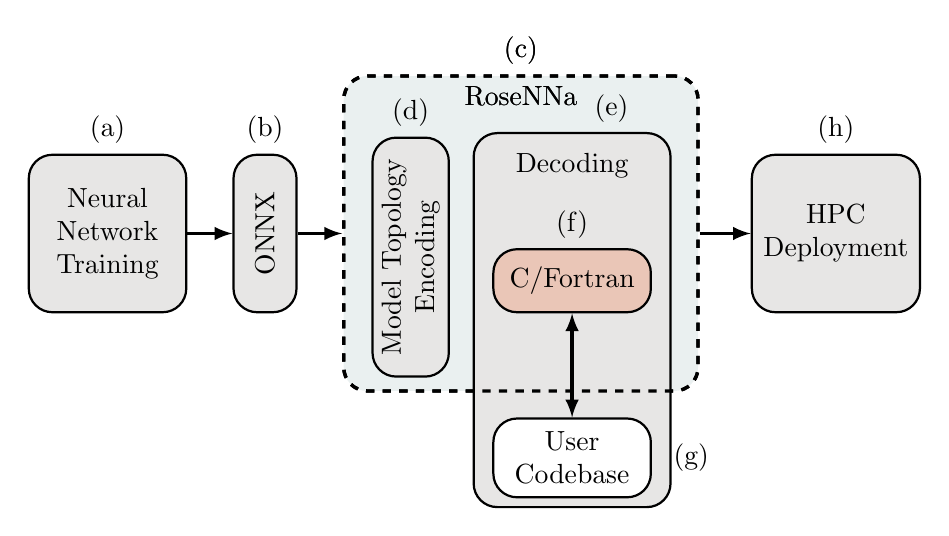
\begin{tikzpicture}[node distance=1cm]
\node (training) [trainingstyle] {Neural Network Training};

\node (onnx) [onnxstyle, below of=training, yshift=-1cm] {ONNX};

\node (border2) [border2style, right of=onnx, xshift=2.25cm,yshift=0cm] {RoseNNa};

\node (mte) [mtestyle, below of=border2, yshift=2.4cm, xshift=-0.3cm] {Model Topology \\ Encoding};

\node (border1) [border1style, right of=mte, xshift=1.05cm, yshift=-0.8cm] {Decoding};

\node (decoding) [decodingstyle, below of=border1,xshift=0cm,yshift=1.5cm] {C/Fortran};

\node (euc) [eucstyle, below of=decoding, yshift=-1.25cm] {User \\ Codebase};

\node (hpc) [hpcstyle, right of=border2, xshift=3cm, yshift=0cm] {HPC \\ Deployment};

\node (border2) [border2style, right of=onnx, xshift=2.25cm,yshift=0cm, fill=none] {RoseNNa};

\draw [arrow] (training) -- (onnx);
\draw [arrow] (onnx) -- (border2);
% \draw [arrow] (mte) -- (3.55,0);
\draw [darrow] (decoding) -- (euc);
\draw [arrow] (border2) -- (hpc);
\end{tikzpicture}
\section{Pipeline Review}
\label{sec:details}
Fig.~\ref{fig:pipeline_supp} depicts the whole pipeline of Hybrid-CSR. From the template meshes $\mathcal{M}_T$, Hybrid-CSR first obtains coarsely deformed cortical meshes $\mathcal{M}_c$, given which, we estimate the positions and normals of upsampled oriented point cloud $\mathcal{O}_{up}$. Then the cortical surfaces $\hat{\mathcal{M}}$ can be reconstructed via poisson surface reconstruction from $\mathcal{O}_{up}$. To fix the topology defects in $\hat{\mathcal{M}}$, we extract non-zero level set from the signed distance grids, obtaining topologically correct meshes $\hat{\mathcal{M}}_{tc'}$, and apply optimization-based diffeomorphic registration to recover the accurate and smooth genus-0 cortical surfaces $\hat{\mathcal{M}}_{tc}$. Lastly, we refine $\hat{\mathcal{M}}_{tc}$ using a learning-based diffeomorphic transformation model, to achieve our final reconstruction results $\hat{\mathcal{M}}_f$.

\section{Implementation Details}
\label{sec:details}

Hybrid-CSR framework is implemented using PyTorch \cite{paszke2019pytorch} and executed on a system equipped with an NVIDIA RTX A6000 GPU and an Intel i7-7700K CPU.

\subsection{Toy Example}
\label{sec:details_toy}

The target contour is controlled by 40 pivot points and the source circle contour includes 200 pivot points. The mesh deformation is modeled via neural fields \cite{xie2022neural}. The positions and normals of oriented point cloud are optimized directly.

\subsubsection{Network Architecture}
\label{sec:toy_net}

To model contour displacements, we encoder positions with random Fourier mapping \cite{tancik2020fourier} and approximate the deformation field with a SIREN \cite{sitzmann2020implicit} model. The gaussian scale and embedding length of position encoding are 5 and 128. The hidden features size and hidden layers number are 256 and 2. Our hybrid method directly optimizes the positions and normals of oriented points. 

\subsubsection{Optimization}

To optimize neural fields for contour deformation, 1000 points with normals are separately sampled from ground truth contour and deformed coutour in each iteration. The loss function consists of geometry-consistency loss and regularization loss. For the geometry-consistency loss, we add up the chamfer distance $\mathcal{L}_{cd}$ and normal distance $\mathcal{L}_{nd}$ between two sets of 1000 sampled oriented points. The regularization loss consists of edge length $\mathcal{L}_{edge}$ \cite{wang2018pixel2mesh}, as well as normal consistency regularization $\mathcal{L}_{nc}$. The total mesh loss is as below:
\begin{equation}
    \mathcal{L} = \mathcal{L}_{cd} + 0.02*\mathcal{L}_{nd} + 0.005*\mathcal{L}_{edge} + 0.005*\mathcal{L}_{nc}
\end{equation}
We apply Adam optimizer \cite{kingma2014adam} with a learning rate of $1e^{-4}$ for 3000 iterations to update the parameters of neural fields.

For the hybrid method, we first uniformly sample 1000 points with normals from the deformed contour obtained above, as initializations. To optimize the positions and normals of oriented points, we minimize the L2 loss between the indicator map reconstructed from the ground truth and the optimized oriented points. We apply Adam optimizer with a learning rate of $3e^{-3}$ for 1000 iterations.

\subsubsection{Results of diffeomorphic transformation}
\label{sec:diff_opt}

\input{fig/toy_example_supp}

In NMF \cite{gupta2020neural}, they present that diffeomorphic transformation can avoid the ``regularizer`s dilemma'', but in our toy experiment, we found neural ode (NODE) \cite{chen2018neural} is not suitable to model large and sharp deformations, as is shown in Fig.~\ref{fig:toy_example_supp}. We model the dynamic function of NODE, i.e., neural velocity fields, using the same neural fields as that for contour deformation and optimize with only chamfer distance and normal distance without any regularization loss, optimized via Adam optimizer with a learning rate of $1e^{-4}$ for 3000 iterations.

\subsection{Coarse Mesh Deformation}
\label{sec:details_cmd}

\subsubsection{Network Architecture}

We apply Vox2Cortex \cite{bongratz2022vox2cortex} to deform template meshes. Same as Vox2Cortex, 
\begin{itemize}
    \item we train the volumetric segmentation branch and mesh deformation branch end-to-end;
    \item volumetric segmentation branch is based on the Res-Unet;
    \item we take four cortical surfaces template as one and use residual GCN-based modules to encode features on graphs;
    \item we use the same feature extraction strategy. That is, in the first step of mesh deformation, the volumetric feature associated with meshes vertices are from the 4th, 5th, 6th and 7th layers of Res-Unet. And in the second step of mesh deformation, the meshes vertices are extracted from the 3rd, 4th, 7th and 8th layers of Res-Unet;
    
\end{itemize}

Different from Vox2Cortex, in the coarse mesh deformation module of Hybrid-CSR 
\begin{itemize}
    \item we deform template meshes in two steps, instead of four steps. In other words, our superiority in performance doesn't come from more steps of surface reconstruction;
    \item In both training and inference, we use smaller templates ($\approx 42000$ vertices per surface).
    
\end{itemize}

\subsubsection{Training}

Same as Vox2Cortex, we apply the loss function composed of voxel loss $\mathcal{L}_vox$, curvature-weighted chamfer loss $\mathcal{L}$, normal distance, laplacian smoothing, normal consistency as well as edge length regularizations. The coarse mesh deformation module as well as segmentation branch are first optimized for 50 epochs and then they will be optimized together with the oriented point cloud estimation module for another 100 epochs. The other implementation details can be found in the supplementary material of Vox2Cortex.

\subsection{Oriented Point Cloud Estimation}
\label{sec:details_opcle}

\subsubsection{Gated Linear Unit (GLU) for Point Estimation} 
% Using GLU, the displacements $\boldsymbol{d}_i$ with an upsample scale of $S$ for each vertex can be estimated as 
% \begin{equation}
%     \boldsymbol{d}_i = (\mathbf{W}_0 \mathbf{f}_i+\mathbf{b}_0) \odot \sigma(\mathbf{W}_1 \mathbf{f}_i+\mathbf{b}_1)
%     \label{eq:glu_point_supp}
% \end{equation}
% where $\mathbf{W}_0, \mathbf{W}_1 \in \mathbb{R}^{(S \times 3) \times d_{out}}$ together with $\mathbf{b}_0, \mathbf{b}_1 \in \mathbb{R}^{(S \times 3)}$ represent linear projections and $\sigma$ represents sigmoid function. The upsampled displacements are then added to the vertex $\boldsymbol{v}_i$ to obtain the point cloud position $\boldsymbol{p}_i^{up} \in \mathbb{R}^{S \times 3}$, written as

Let $S$ denote the upsample ratio, $\boldsymbol{p}_i^{up} \in \mathbb{R}^{S \times 3}$ denote the position of upsampled oriented point clouds, $\boldsymbol{v}_i^{up} \in \mathbb{R}^{S \times 3}$ denote the vertex of deformed meshes repeated by $S$ times and $\boldsymbol{p}_i^{up}$ denote the upsampled displacements of vertex $\boldsymbol{v}_i$. 
Let's also define the intermediate position of upsampled oriented point clouds as $\boldsymbol{p'}_i^{up} \in \mathbb{R}^{S \times 3}$, such that 
\begin{equation}
    \boldsymbol{p}_i^{up} = (1-\boldsymbol{m}_i) \odot \boldsymbol{v}_i^{up} + \boldsymbol{m}_i \odot \boldsymbol{p'}_i^{up}
    \label{eq:point_displace_supp_1}
\end{equation}
where each dimension of $\boldsymbol{m}_i$ is between 0 and 1, controlling the ``confidence'' of the intermediate results. 
% If $m_i$, the intermediate positions are the final positions. While $m_i=0$, the predicted intermediate positions are most unreliable, thus we take the final positions as $\boldsymbol{v}_i^{up}$. 
We can represent $\boldsymbol{p'}_i^{up}$ as $\boldsymbol{v}_i^{up} + \boldsymbol{d'}_i$, where $\boldsymbol{d'}_i^{up}$ is intermediate displacement associated with upsampled vertex $\boldsymbol{v}_i^{up}$. Therefore, the Eq.~\ref{eq:point_displace_supp_1} can be rewritten as:
\begin{equation}
    \boldsymbol{p}_i^{up} = \boldsymbol{v}_i^{up} + \boldsymbol{m}_i \odot \boldsymbol{d'}_i^{up}
    \label{eq:point_displace_supp_2}
\end{equation}
As we have demonstrated in the main paper, using GLU, the displacements can be written as $\boldsymbol{d_i} = (\mathbf{W}_0 \mathbf{f}_i+\mathbf{b}_0) \odot \sigma(\mathbf{W}_1 \mathbf{f}_i+\mathbf{b}_1)$. Then, we have
\begin{equation}
    (\mathbf{W}_0 \mathbf{f}_i+\mathbf{b}_0) \odot \sigma(\mathbf{W}_1 \mathbf{f}_i+\mathbf{b}_1) = \boldsymbol{m}_i \odot \boldsymbol{d'}_i^{up}
    \label{eq:point_displace_supp_2}
\end{equation}
Thus, we suppose $\mathbf{W}_0 \in \mathbb{R}^{(S \times 3) \times (d_{out} + S \times 3)}$ and $\mathbf{b}_0 \in \mathbb{R}^{(S \times 3)}$ modulate the displacement vector, while $\mathbf{W}_1 \in \mathbb{R}^{(S \times 3) \times (d_{out} + S \times 3)}$ and $\mathbf{b}_1 \in \mathbb{R}^{(S \times 3)}$ modulate the ``confidence '' of the predicted displacement vector. In our experiments, $S=7$ and $d_{out}=64$. 

\subsubsection{Network Architecture for Normal Estimation} 
\input{fig/normal_estimation}

As is shown in Fig.~\ref{fig:normal_est_supp}, GCN is used to encode features on graph and GLU is used to estimate normals of upsampled positions. The input of GCN is the concatenation of grouped positions, grouped image features associated with points and graph feature generated by the previous GCN layer. The positions and associated features will be grouped into the same node if they are displaced from the same vertices. We sample the image features from the 2nd, 3rd, 8th and 9th layers of Res-Unet given the point positions via linear interpolation, and the channel number of these volumetric features are 32, 64, 16 and 8. The graph feature from the previous layer is in length of 64. Thus, the input feature channel number of GCN is $S*(3+(32+64+16+8)) + 64 = 925$ and the output feature channel number is 64. 

The output of GCN concatenated with the grouped positions is taken as the input of GLU, whose input feature channel number is therefore $64+S*3=85$. The output of GLU is the normals of upsampled point clouds, thus the output channel number is $S*3=21$.


\subsubsection{Training}

We apply weighted mean square error $\mathcal{L}_{DPSR}$ to measure the difference between predicted and ground truth indicator grids. The weight map is the smoothed edge map of the ground truth indicator grid. Together with mesh-based loss proposed in Vox2Cortex, $\mathcal{L}_{DPSR}$ is used to optimize Hybrid-CSR in an end-to-end manner for additional 100 epochs. The parameters of oriented point cloud estimation module are optimized via an Adam optimizer of a learning rate of $5e^{-5}$.

\subsection{Topology Correction}
\label{sec:details_topo}

We model the neural velocity fields $\mathcal{F}_{\theta}$, using the same network architecture as described in Sec.~\ref{sec:toy_net} and Sec.~\ref{sec:diff_opt}. Other implementation details are included in the main paper. 

Different from the toy example, in the procedure of topology correction, the source surface $\hat{\mathcal{M}}_{tc'}$ and target surface $\hat{\mathcal{M}}_{tc}$ have already been well-aligned, so that diffeomorphic transformation optimized by chamfer distance is able to provide accurate surface registration performance.

\subsection{Surface Refinement}
\label{sec:details_refine}

The network architecture of surface refinement is the same as CortexODE \cite{ma2022cortexode}. But there are some differences in training pial surface refinement model. In the original CortexODE, they learn to map the ground truth WM surface to the ground truth pial surface. Since the ground truth WM and pial surface share the same topology, they can train with the L2 distance. However, during inference, the source surface is the predicted WM surface obtained from Marching Cubes so there exists a discrepancy between inference and training. Instead, we learn to map the topological correct pial surface to the ground truth pial surface, supervised by chamfer distance. And during inference, the initial pial surface is also generated by the topology correction procedure. In terms of other implementation details, we follow the original CortexODE.

% \subsection{Results of Pre-trained CorticalFlow++}
% \label{sec:cortical}

% \begin{table*}[!ht]
\centering
\resizebox{\linewidth}{!}{%
\begin{tabular}{lcccccccccccc} 
\toprule
               & \multicolumn{3}{c}{Left Pial} 
               & \multicolumn{3}{c}{Left WM} 
               & \multicolumn{3}{c}{Right Pial} 
               & \multicolumn{3}{c}{Right WM}  \\ 
               
\cmidrule(lr){2-4}\cmidrule(lr){5-7}\cmidrule(lr){8-10}\cmidrule(lr){11-13}
          Dataset & ASSD  & NC    & SI     & ASSD & NC    & SI & ASSD & NC    & SI & ASSD & NC    & SI             \\ 
\midrule          
ADNI  & .178   & .938  & .063  & .214  & .943  & .013  & .174  & .938  & .086   & .212 & .942 & .026            \\
OASIS & .326   & .913  & .147  & .225  & .937  & .054  & .318  & .913  & .192   & .227 & .935 & .076           \\
\bottomrule
\end{tabular}
}
\caption{
% 
\textbf{Cortical Surface Reconstruction from Pre-trained CorticalFlow++}
% 
} % \caption
\label{tab:pre-trained_cfpp}
\end{table*}

% CorticalFlow++ \cite{santa2022corticalflow++} provided model checkpoints trained on a large ADNI dataset (over $3,876$ scans) and we present the performance of pre-trained CorticalFlow++ in Tab.~\ref{tab:pre-trained_cfpp}. We didn't put it in the main paper for two reasons: (1) all the other methods are trained on smaller-size data and (2) the test ADNI data we used for evaluation might be included in the training samples of the pre-trained CorticalFlow++ model.

\section{Visual Comparisons with Competing Methods}
\label{sec:vis_comp}
\input{fig/vis_comp}

In this section, we provide the comprehensive visual comparison between our Hybrid-CSR and other competing methods, including Vox2Cortex \cite{bongratz2022vox2cortex}, CorticalFlow++ \cite{santa2022corticalflow++}, CortexODE \cite{ma2022cortexode} as well as DeepCSR \cite{cruz2021deepcsr}. From Fig.~\ref{fig:vis_comp}, we can see our proposed Hybrid-CSR in general can generate surfaces in lighter colors, i.e., smaller point-to-surface distances, compared with other methods.